% Source problem: 2011ap_exam.pdf, PDF pp. 10--11.
\documentclass[11pt,a4paper]{article}
\usepackage[margin=24mm]{geometry}
\usepackage{fontspec}
\usepackage{xeCJK}
\setCJKmainfont{HaranoAjiMincho-Regular.otf}
\setCJKsansfont{HaranoAjiGothic-Medium.otf}
\usepackage{amsmath,amssymb}
\usepackage{tikz}
\usetikzlibrary{arrows.meta}
\setlength{\parindent}{1em}
\setlength{\parskip}{0.35em}
\renewcommand{\figurename}{図}
\title{物理工学専攻 院試解答集\\2011年 物理学II 第4問}
\author{政岡凜太郎}
\date{}
\begin{document}
\maketitle

\section*{[1] 周期境界条件}
周期境界条件では、原子軌道の添字 $j$ と $j+M$ を同一視する。
したがって、同じ軌道に掛かるBloch係数も一致しなければならず、
\begin{equation}
  e^{ik(j+M)a}=e^{ikja},\qquad e^{ikMa}=1
\end{equation}
となる。この条件の下でBloch和は $\psi_k(x+Ma)=\psi_k(x)$ を満たす。
従って許される波数は
\begin{equation}
  \boxed{k=\frac{2\pi l}{Ma}\quad(l\in\mathbb Z)}.
\end{equation}
第一ブリルアン領域内では隣り合う波数の間隔は $2\pi/(Ma)$ である。

\section*{[2] 単元素鎖のエネルギー分散}
問題文のシュレーディンガー方程式(1)に $\psi_k$ を代入し、$\phi_A^*(x)$ を掛けて積分する。運動エネルギー演算子を $T=-\hbar^2\partial_x^2/(2m)$ と書く。孤立原子の方程式から $\langle\phi_A|T+u(x)|\phi_A\rangle=E_A$ となる。隣接する二つのA原子イオンのポテンシャルはそれぞれ $\beta$ を与え、オンサイトのエネルギーは $E_A+2\beta$ である。

右隣の軌道については、その原子の孤立方程式と軌道の直交性から
\begin{equation}
 \int\phi_A^*(x)[T+u(x-a)]\phi_A(x-a)\,dx
 =E_A\int\phi_A^*(x)\phi_A(x-a)\,dx=0.
\end{equation}
したがって全ポテンシャルのうち原点の $u(x)$ が残す行列要素が、問題で定義された $\gamma$ である。左隣も同様に $\gamma$ を与え、両者にはBloch位相 $e^{ika}$ と $e^{-ika}$ が付く。列挙外の積分は無視できるので
\begin{align}
  E(k)&=E_A+2\beta+\gamma(e^{ika}+e^{-ika})\\
      &=\boxed{E_A+2\beta+2\gamma\cos(ka)}.
\end{align}

\section*{[3] 第一ブリルアン領域と安定性}
孤立原子の準位 $E_A$ は、真空準位を基準に束縛状態なら負である。隣接イオンの引力ポテンシャルによる対角シフト $2\beta$ も安定な結晶では一般に負となる。移動積分の符号はバンド底の位置を決める。安定な結合性の底端が $k=0$ にある場合は $\gamma<0$ で、バンド底 $E_A+2\beta+2\gamma$ は上端 $E_A+2\beta-2\gamma$ より低い。バンド幅は $4|\gamma|$ である。

\begin{figure}[htbp]
\centering
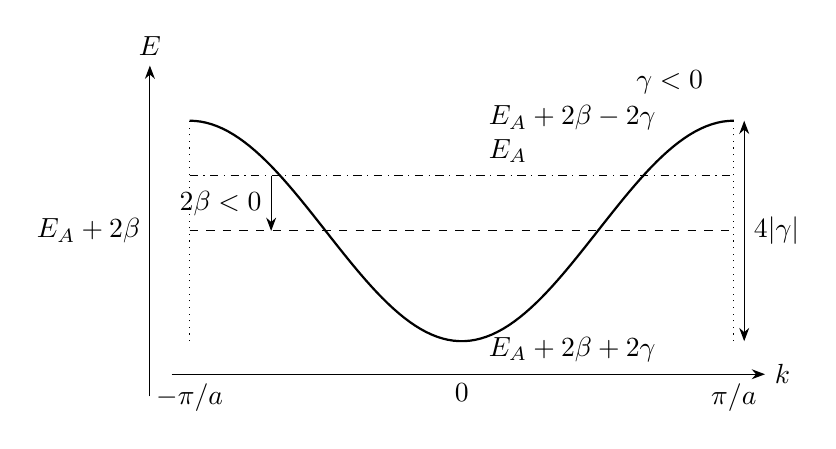
\begin{tikzpicture}[>=Stealth,x=1.1cm,y=0.7cm]
  \pgfmathsetmacro{\gammaVal}{-1}
  \pgfmathsetmacro{\betaVal}{-0.5}
  \pgfmathsetmacro{\gammaMagnitude}{abs(\gammaVal)}
  \pgfmathsetmacro{\atomicLevel}{-2*\betaVal/\gammaMagnitude}
  \pgfmathsetmacro{\axisBase}{-2.6}
  \pgfmathsetmacro{\axisRight}{pi+0.36}
  \draw[->] (-3.6,-3.0) -- (-3.6,3.0) node[above] {$E$};
  \draw[->] (-3.35,\axisBase) -- (\axisRight,\axisBase) node[right] {$k$};
  \draw[dashed] (-pi,0) -- (pi,0);
  \draw[dash dot] (-pi,\atomicLevel) -- (pi,\atomicLevel);
  \node[anchor=west] at (0.2,\atomicLevel+0.45) {$E_A$};
  \draw[->] (-2.2,\atomicLevel) -- (-2.2,0) node[midway,left] {$2\beta<0$};
  \draw[<->] (pi+0.12,-2) -- (pi+0.12,2) node[midway,right] {$4|\gamma|$};
  \draw[thick,samples=100] plot[domain=-180:180] ({\x*pi/180},{2*\gammaVal*cos(\x)});
  \draw[dotted] (-pi,-2) -- (-pi,2);
  \draw[dotted] (pi,-2) -- (pi,2);
  \node[below] at (-pi,\axisBase) {$-\pi/a$};
  \node[below] at (0,\axisBase) {$0$};
  \node[below] at (pi,\axisBase) {$\pi/a$};
  \node[left] at (-3.6,0) {$E_A+2\beta$};
  \node[anchor=west] at (0.2,-2.15) {$E_A+2\beta+2\gamma$};
  \node[anchor=west] at (0.2,2.05) {$E_A+2\beta-2\gamma$};
  \node at (2.4,2.7) {$\gamma<0$};
\end{tikzpicture}
\caption{単元素鎖の分散。縦方向は $|\gamma|$ を単位とする。表示例では $\gamma=-|\gamma|$ と $2\beta=-|\gamma|$ を選び、他のエネルギー比は示していない。}
\end{figure}

\section*{[4] 電子と正孔の有効質量}
まず[3]の図と同じ $\gamma<0$ の場合を考える。
一つの軌道にスピンの異なる2個の電子を収容できるので、単位胞あたりの占有数2が満占有に対応する。
バンド端近傍の曲率は
\begin{equation}
  \frac{d^2E}{dk^2}=-2\gamma a^2\cos(ka).
\end{equation}
基底状態または低温の低エネルギーキャリアを考えると、平均占有数が1より十分小さいときの電子はバンド底 $k=0$ の近くに入る。よって
\begin{equation}
  \boxed{m_e^*=\frac{\hbar^2}{E''(0)}
  =\frac{\hbar^2}{-2\gamma a^2}>0.}
\end{equation}
同じ低エネルギー条件のもとで占有数が2に近いときは、バンド上端 $k=\pi/a$ 近くの空状態を正孔として扱う。電子の曲率は $E''(\pi/a)=2\gamma a^2<0$ なので、正孔の質量はその負号付き逆数で
\begin{equation}
  \boxed{m_h^*=-\frac{\hbar^2}{E''(\pi/a)}
  =-\frac{\hbar^2}{2\gamma a^2}>0.}
\end{equation}
この最近接余弦バンドでは両者の大きさが等しい。正孔質量の負号は、電子バンド頂の負曲率を正の正孔質量に変換するために必要である。
$\gamma>0$ ではバンド底と上端の位置が入れ替わり、電子は $k=\pi/a$、正孔は $k=0$ の近くで評価する。
したがって $\gamma\ne0$ でのキャリア質量は、どちらも $\hbar^2/(2|\gamma|a^2)$ である。
$\gamma=0$ ではバンドが平坦となり、有限の曲率から質量を求めるこの式は使えない。

\section*{[5] 二原子分子鎖の固有値方程式}
一単位胞の基底を $\phi_A,\phi_B$ とする。原子Aの対角要素は $E_A+2\beta$、隣の単位胞にあるA軌道との移動要素は[2]とBloch和により $2\gamma\cos(ka)$ となる。B軌道の対角要素は $E_B$。A–B間の要素にも運動エネルギーの寄与がある。[2]で定義した $T$ を用い、同一分子内の軌道の重なりを $S_{AB}=\langle\phi_A|\phi_B\rangle$ と置く。原問では列挙されていない重なり積分を無視するので $S_{AB}\simeq0$ である。孤立A原子の方程式 $(T+u)\phi_A=E_A\phi_A$ とHermite性から
\begin{align}
  \langle\phi_A|T+u|\phi_B\rangle&=E_A S_{AB},\\
  \langle\phi_A|T+u+w|\phi_B\rangle
    &=E_A S_{AB}+\langle\phi_A|w|\phi_B\rangle\simeq\delta.
\end{align}
孤立B原子の方程式から評価しても、同じ要素は $E_B S_{AB}+\langle\phi_A|u|\phi_B\rangle\simeq\delta$ となる。従って二つの等しいポテンシャル積分は、運動項を含む行列要素をそれぞれ評価するものである。係数 $c_k,d_k$ は
\begin{equation}
  \boxed{
  \begin{pmatrix}
    E_A+2\beta+2\gamma\cos(ka)&\delta\\
    \delta&E_B
  \end{pmatrix}
  \begin{pmatrix}c_k\\d_k\end{pmatrix}
  =E(k)\begin{pmatrix}c_k\\d_k\end{pmatrix}.}
\end{equation}
ここで行列はHermiteであり、固有値は実数となる。

\section*{[6] 混成バンド}
\begin{equation}
  \Delta=E_A-E_B+2\beta
\end{equation}
と置く。固有値方程式の行列式から
\begin{align}
  0&=[E_A+2\beta+2\gamma\cos(ka)-E][E_B-E]-\delta^2.
\end{align}
\begin{equation}
  \boxed{\begin{aligned}
  E_{\pm}(k)&=\frac{E_A+E_B}{2}+\beta+\gamma\cos(ka)\\
  &\quad\pm\sqrt{\left(\frac{\Delta}{2}+\gamma\cos(ka)\right)^2+\delta^2}.
  \end{aligned}}
\end{equation}

まず $\delta=0$ なら、A由来の余弦バンド $E_A+2\beta+2\gamma\cos(ka)$ と、分散のないB準位 $E_B$ が交差する。交差条件は $\Delta+2\gamma\cos(ka)=0$ である。$|\Delta|\ll|\gamma|$ では交差点が第一ブリルアン領域内にあり、$\Delta=0$ なら $ka=\pm\pi/2$。一方 $|\Delta|\gg|\gamma|$ では両バンドの中心エネルギー差がAバンドの半幅より十分大きく、交差しない。

$\delta\ne0$ はAとBの混成を生む。交差点近傍では固有値が分裂し、直接ギャップは $2|\delta|$ となる。$|\Delta|\gg|\gamma|$ では未混成準位差 $|\Delta+2\gamma\cos(ka)|$ が全波数で $|\delta|$ より十分大きい。固有値方程式の二行から
\begin{equation}
 \delta d_k=[E(k)-E_A-2\beta-2\gamma\cos(ka)]c_k,
 \qquad \delta c_k=[E(k)-E_B]d_k
\end{equation}
となる。Bに近い枝では $|c_k/d_k|\simeq|\delta/(\Delta+2\gamma\cos(ka))|\ll1$、Aに近い枝では同様に $|d_k/c_k|\ll1$ だから、各枝は主に元のAまたはB軌道の性質を保つ。また固有値のずれは
\begin{equation}
 \sqrt{\frac{[\Delta+2\gamma\cos(ka)]^2}{4}+\delta^2}
 -\frac{|\Delta+2\gamma\cos(ka)|}{2}
 \simeq\frac{\delta^2}{|\Delta+2\gamma\cos(ka)|}
\end{equation}
と小さい。これは下図の大離調での弱い準位移動にも対応する。

\begin{figure}[htbp]
\centering
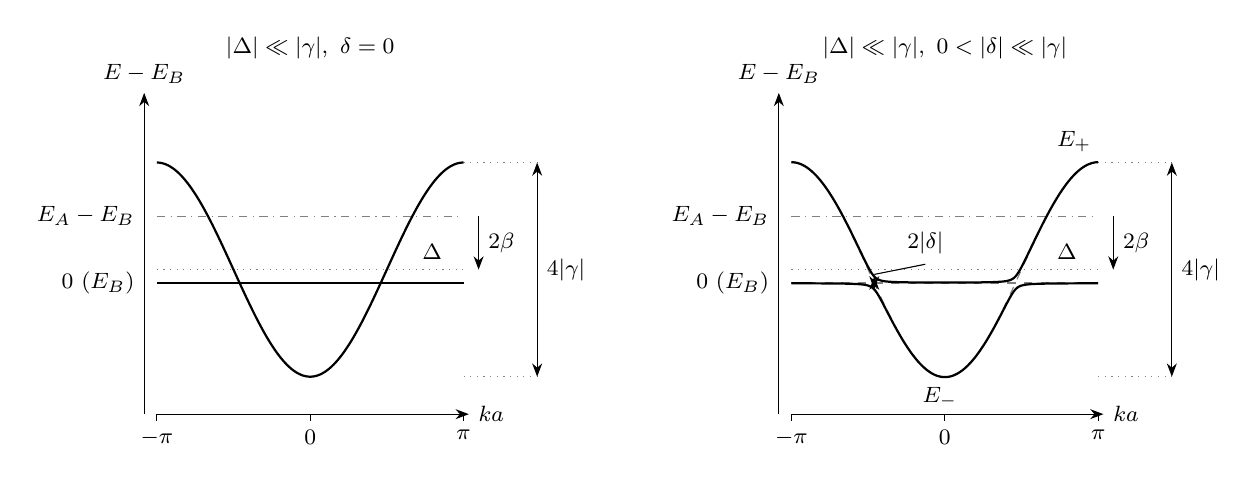
\begin{tikzpicture}[>=Stealth,x=0.62cm,y=0.68cm,font=\footnotesize]
\pgfmathsetmacro{\gammaVal}{-1}
\pgfmathsetmacro{\gammaMagnitude}{abs(\gammaVal)}
\pgfmathsetmacro{\betaVal}{-0.5}
\pgfmathsetmacro{\mixing}{0.12}
\pgfmathsetmacro{\detuning}{0.25}
\pgfmathsetmacro{\atomicA}{\detuning-2*\betaVal}
\pgfmathsetmacro{\aBottom}{\detuning-2*\gammaMagnitude}
\pgfmathsetmacro{\aTop}{\detuning+2*\gammaMagnitude}
\begin{scope}[shift={(0,0)}]
  \draw[->] (-3.4,-2.45)--(-3.4,3.55);
  \node[above] at (-3.4,3.55) {$E-E_B$};
  \draw[->] (-pi,-2.45)--(3.25,-2.45) node[right] {$ka$};
  \foreach \k/\label in {-1/{-\pi},0/0,1/\pi} {\draw ({\k*pi},-2.45)--++(0,-0.12) node[below] {$\label$};}
  \node[above] at (0,4.0) {$|\Delta|\ll|\gamma|,\ \delta=0$};
  \draw[gray,dash dot] (-pi,\atomicA)--(pi,\atomicA);
  \node[left] at (-3.4,\atomicA) {$E_A-E_B$};
  \draw[gray,dotted] (-pi,\detuning)--(3.15,\detuning);
  \node[above] at (2.5,\detuning) {$\Delta$};
  \draw[gray,dashed] (-pi,0)--(pi,0);
  \node[left] at (-3.4,0) {$0\ (E_B)$};
  \draw[->] (3.45,\atomicA)--(3.45,\detuning)
    node[midway,right] {$2\beta$};
  \draw[dotted,gray] (pi,\aBottom)--(4.65,\aBottom);
  \draw[dotted,gray] (pi,\aTop)--(4.65,\aTop);
  \draw[<->] (4.65,\aBottom)--(4.65,\aTop)
    node[midway,right] {$4|\gamma|$};
  \draw[thick,samples=140] plot[domain=-180:180]
    ({\x*pi/180},{\detuning+2*\gammaVal*cos(\x)});
  \draw[thick] (-pi,0)--(pi,0);
\end{scope}
\begin{scope}[shift={(13,0)}]
  \draw[->] (-3.4,-2.45)--(-3.4,3.55);
  \node[above] at (-3.4,3.55) {$E-E_B$};
  \draw[->] (-pi,-2.45)--(3.25,-2.45) node[right] {$ka$};
  \foreach \k/\label in {-1/{-\pi},0/0,1/\pi} {\draw ({\k*pi},-2.45)--++(0,-0.12) node[below] {$\label$};}
  \node[above] at (0,4.0) {$|\Delta|\ll|\gamma|,\ 0<|\delta|\ll|\gamma|$};
  \draw[gray,dash dot] (-pi,\atomicA)--(pi,\atomicA);
  \node[left] at (-3.4,\atomicA) {$E_A-E_B$};
  \draw[gray,dotted] (-pi,\detuning)--(3.15,\detuning);
  \node[above] at (2.5,\detuning) {$\Delta$};
  \draw[gray,dashed] (-pi,0)--(pi,0);
  \node[left] at (-3.4,0) {$0\ (E_B)$};
  \draw[->] (3.45,\atomicA)--(3.45,\detuning)
    node[midway,right] {$2\beta$};
  \draw[dotted,gray] (pi,\aBottom)--(4.65,\aBottom);
  \draw[dotted,gray] (pi,\aTop)--(4.65,\aTop);
  \draw[<->] (4.65,\aBottom)--(4.65,\aTop)
    node[midway,right] {$4|\gamma|$};
  \draw[gray,dashed,samples=140] plot[domain=-180:180]
    ({\x*pi/180},{\detuning+2*\gammaVal*cos(\x)});
  \draw[thick,samples=180] plot[domain=-180:180]
    ({\x*pi/180},{(\detuning+2*\gammaVal*cos(\x))/2-sqrt(((\detuning+2*\gammaVal*cos(\x))/2)^2+\mixing^2)});
  \draw[thick,samples=180] plot[domain=-180:180]
    ({\x*pi/180},{(\detuning+2*\gammaVal*cos(\x))/2+sqrt(((\detuning+2*\gammaVal*cos(\x))/2)^2+\mixing^2)});
  \pgfmathsetmacro{\crossing}{-acos(-\detuning/(2*\gammaVal))*pi/180}
  \draw[<->] (\crossing,-\mixing)--(\crossing,\mixing);
  \draw[thin] (\crossing,\mixing+0.04)--(-0.4,0.35);
  \node[above] at (-0.4,0.35) {$2|\delta|$};
  \node[above] at (2.65,\aTop+0.02) {$E_+$};
  \node[below] at (-0.1,\aBottom-0.02) {$E_-$};
\end{scope}
\end{tikzpicture}
\vspace{0.8em}

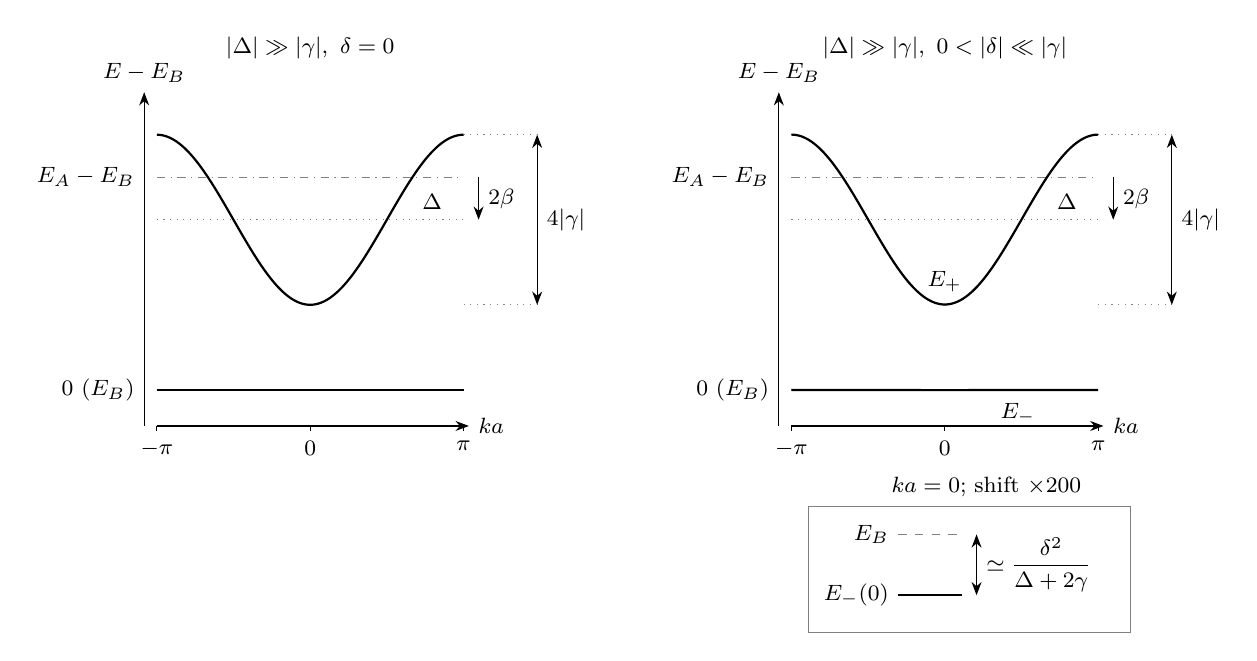
\begin{tikzpicture}[>=Stealth,x=0.62cm,y=0.54cm,font=\footnotesize]
\pgfmathsetmacro{\gammaVal}{-1}
\pgfmathsetmacro{\gammaMagnitude}{abs(\gammaVal)}
\pgfmathsetmacro{\betaVal}{-0.5}
\pgfmathsetmacro{\mixing}{0.12}
\pgfmathsetmacro{\detuning}{4}
\pgfmathsetmacro{\atomicA}{\detuning-2*\betaVal}
\pgfmathsetmacro{\aBottom}{\detuning-2*\gammaMagnitude}
\pgfmathsetmacro{\aTop}{\detuning+2*\gammaMagnitude}
\begin{scope}[shift={(0,0)}]
  \draw[->] (-3.4,-0.85)--(-3.4,7.0);
  \node[above] at (-3.4,7.0) {$E-E_B$};
  \draw[->] (-pi,-0.85)--(3.25,-0.85) node[right] {$ka$};
  \foreach \k/\label in {-1/{-\pi},0/0,1/\pi} {\draw ({\k*pi},-0.85)--++(0,-0.12) node[below] {$\label$};}
  \node[above] at (0,7.55) {$|\Delta|\gg|\gamma|,\ \delta=0$};
  \draw[gray,dash dot] (-pi,\atomicA)--(pi,\atomicA);
  \node[left] at (-3.4,\atomicA) {$E_A-E_B$};
  \draw[gray,dotted] (-pi,\detuning)--(3.15,\detuning);
  \node[above] at (2.5,\detuning) {$\Delta$};
  \draw[gray,dashed] (-pi,0)--(pi,0);
  \node[left] at (-3.4,0) {$0\ (E_B)$};
  \draw[->] (3.45,\atomicA)--(3.45,\detuning)
    node[midway,right] {$2\beta$};
  \draw[dotted,gray] (pi,\aBottom)--(4.65,\aBottom);
  \draw[dotted,gray] (pi,\aTop)--(4.65,\aTop);
  \draw[<->] (4.65,\aBottom)--(4.65,\aTop)
    node[midway,right] {$4|\gamma|$};
  \draw[thick,samples=140] plot[domain=-180:180]
    ({\x*pi/180},{\detuning+2*\gammaVal*cos(\x)});
  \draw[thick] (-pi,0)--(pi,0);
\end{scope}
\begin{scope}[shift={(13,0)}]
  \draw[->] (-3.4,-0.85)--(-3.4,7.0);
  \node[above] at (-3.4,7.0) {$E-E_B$};
  \draw[->] (-pi,-0.85)--(3.25,-0.85) node[right] {$ka$};
  \foreach \k/\label in {-1/{-\pi},0/0,1/\pi} {\draw ({\k*pi},-0.85)--++(0,-0.12) node[below] {$\label$};}
  \node[above] at (0,7.55) {$|\Delta|\gg|\gamma|,\ 0<|\delta|\ll|\gamma|$};
  \draw[gray,dash dot] (-pi,\atomicA)--(pi,\atomicA);
  \node[left] at (-3.4,\atomicA) {$E_A-E_B$};
  \draw[gray,dotted] (-pi,\detuning)--(3.15,\detuning);
  \node[above] at (2.5,\detuning) {$\Delta$};
  \draw[gray,dashed] (-pi,0)--(pi,0);
  \node[left] at (-3.4,0) {$0\ (E_B)$};
  \draw[->] (3.45,\atomicA)--(3.45,\detuning)
    node[midway,right] {$2\beta$};
  \draw[dotted,gray] (pi,\aBottom)--(4.65,\aBottom);
  \draw[dotted,gray] (pi,\aTop)--(4.65,\aTop);
  \draw[<->] (4.65,\aBottom)--(4.65,\aTop)
    node[midway,right] {$4|\gamma|$};
  \draw[gray,dashed,samples=140] plot[domain=-180:180]
    ({\x*pi/180},{\detuning+2*\gammaVal*cos(\x)});
  \draw[thick,samples=180] plot[domain=-180:180]
    ({\x*pi/180},{(\detuning+2*\gammaVal*cos(\x))/2-sqrt(((\detuning+2*\gammaVal*cos(\x))/2)^2+\mixing^2)});
  \draw[thick,samples=180] plot[domain=-180:180]
    ({\x*pi/180},{(\detuning+2*\gammaVal*cos(\x))/2+sqrt(((\detuning+2*\gammaVal*cos(\x))/2)^2+\mixing^2)});
  \node[above] at (0,\aBottom+0.08) {$E_+$};
  \node[below] at (1.5,-0.08) {$E_-$};
  \pgfmathsetmacro{\bShift}{sqrt((\detuning+2*\gammaVal)^2/4+\mixing^2)-(\detuning+2*\gammaVal)/2}
  \pgfmathsetmacro{\zoom}{200}
  \pgfmathsetmacro{\zoomTop}{-3.4}
  \pgfmathsetmacro{\zoomBottom}{\zoomTop-\zoom*\bShift}
  \draw[gray] (-2.8,-5.7) rectangle (3.8,-2.75);
  \node[above] at (0.85,-2.75) {$ka=0$; shift $\times200$};
  \draw[gray,dashed] (-0.95,\zoomTop)--(0.35,\zoomTop);
  \node[left] at (-0.95,\zoomTop) {$E_B$};
  \draw[thick] (-0.95,\zoomBottom)--(0.35,\zoomBottom);
  \node[left] at (-0.95,\zoomBottom) {$E_-(0)$};
  \draw[<->] (0.65,\zoomBottom)--(0.65,\zoomTop)
    node[midway,right] {$\simeq\dfrac{\delta^2}{\Delta+2\gamma}$};
\end{scope}
\end{tikzpicture}
\caption{混成の有無と離調の大小による分散。エネルギーは $|\gamma|$ を単位とし、$E_B$ を基準とする。全図で $\gamma=-1$、$\beta=-0.5$、小離調は $\Delta=0.25$、大離調は $\Delta=4$ とした。有限混成の二図はともに $\delta=0.12$。実線は固有エネルギー、破線は未混成AバンドとB準位、一点鎖線は孤立A準位、点線はAバンド中心を示す。矢印 $2\beta$ は孤立A準位から中心への移動、$4|\gamma|$ は未混成Aバンドの幅である。右上は交差波数でのギャップ、右下の枠内は $ka=0$ でのB由来準位の移動を縦に200倍拡大した図で、実線の位置は厳密な固有値から計算した。$\Delta<0$ の大離調では上下のバンド順が逆になる。}
\end{figure}

\end{document}
